\section{Integration with differential forms}

What we've discussed so far has shown that out operator $d$ takes a scalar field $f$
and produces a covector field $df$ which is the level sets of $f$ oriented towards the positive
values of $f$.\\
And this covector field $df$ can behave like a function that acts on vectors.\\
If applied to a vector $\vec{v}$, we think about zooming on the covector at the point of $\vec{v}$ and 
count how many times the vector piereces to get the output.\\

So this reinterpretation of the operator $d$ gives us covector fields which are also called differential forms.
How does this relate back to the differential we see in integrals, which represents a small change in the varibale, for 
example $dx$?\\

The short answer is that, every single integral involves:

\begin{itemize}
    \item a \begingroup\color{red}differential form (covector field)\endgroup
    \item a \begingroup\color{blue}path\endgroup
\end{itemize}

\begin{equation}
    \int_{\begingroup\color{blue}a\endgroup}^{\begingroup\color{blue}b\endgroup}
    \begingroup\color{red}f(x)dx\endgroup
\end{equation}

The result of the integral is just the number of $\begingroup\color{red}\text{covector stacks}\endgroup$ pierced by the \begingroup\color{blue}path\endgroup.\\

To prove this, we're going to explore a couple of examples from Physics, but first let's quickly review two important
theorems from calculus:

\begin{itemize}
    \item Fundamental Theorem of Calculus
    \begin{align*}
        \int_a^b f(x)dx = F(b) - F(a)\\
        \int_a^b \frac{dF}{dx}dx = F(b) - F(a)
    \end{align*}
    \item Gradient Theorem
    \begin{align*}
        \int_{P[a,b]} \grad{F} \cdot dr= F(b) - F(a)
    \end{align*}
\end{itemize}

Both of them involve integrals over a path from a to b, where the integral itself 
only depends on the values at the endpoints.\\
We're going to prove the Gradient theorem to show why differential forms are strictly tied to integrals.\\

Recall what work is in physics, it's the application of a force to an object along some distance, the force dot 
product with the displacement vector:

\begin{equation}
    W = \begingroup\color{cyan}\vec{F}\endgroup \cdot \begingroup\color{violet}\vec{R}\endgroup
\end{equation}

The dot product actually tells us how much of the force was used to move the object along the displacement vector.\\
Let's say that we have some force vector defined as:

\begin{equation}
    \begingroup\color{cyan}\vec{F}\endgroup = 2\begingroup\color{blue}\vec{e_1}\endgroup + 1\begingroup\color{blue}\vec{e_2}\endgroup
\end{equation}

\begin{center}
\pgfplotsset{compat=1.17}
 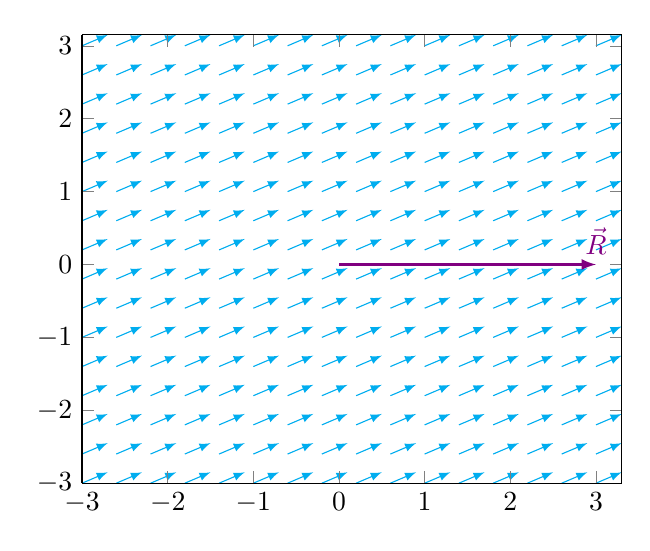
\begin{tikzpicture}
 \begin{axis}[%
  view     = {0}{90}, % for a view 'from above'
  domain   = -3:3,
  y domain = -3:3,
  xtick    = {-3,...,3},
  ytick    = {-3,...,3},
]
\addplot3[cyan, quiver={u=2, v=1, scale arrows=0.15}, samples=16, -latex] (x,y,0);
% Vector along x-axis with length R=3
\addplot[
  violet, thick, -latex
] coordinates {(0,0) (3,0)} 
node[pos=1, above] {$\begingroup\color{violet}\vec{R}\endgroup$}; % label at the tip
\end{axis}
\end{tikzpicture}
\end{center}

And our vector giving us the direction is:

\begin{equation}
    \begingroup\color{violet}\vec{R}\endgroup = 3\begingroup\color{blue}\vec{e_1}\endgroup + 0\begingroup\color{blue}\vec{e_2}\endgroup
\end{equation}

The total work would be $W = \begingroup\color{cyan}\vec{F}\endgroup \cdot \begingroup\color{violet}\vec{R}\endgroup = 6$ Joules\\

Now, for a bit more meaningful example, consider the force field due to the gravitational field that the 
earch exercit on a smaller mass m, at a distance $\begingroup\color{violet}\vec{R}\endgroup$:

\begin{equation}
    \begingroup\color{cyan}\vec{F}\endgroup = \frac{GMm}{\|\begingroup\color{violet}\vec{R}^2\endgroup\|} (-\begingroup\color{red}\vec{e_r}\endgroup)
\end{equation}

Giving a curved path with an object traveling along, how do we compute the work done on this object, by
the gravitational field. The formula we used before is not valid here, as the force field 
is different at every point in space, and the path we're traveling along is curved.\\

We actually need to perform an integration along the path like:

\begin{equation}
    W = \int_{\begingroup\color{orange}P\endgroup} \begingroup\color{cyan}\vec{F}_G\endgroup \cdot d\begingroup\color{violet}\vec{R}\endgroup
\end{equation}

This $d\begingroup\color{violet}\vec{R}\endgroup$, what it really is, it's just a short way of seeing $\frac{d\begingroup\color{violet}\vec{R}\endgroup}{d\begingroup\color{brown}\lambda\endgroup} d\begingroup\color{brown}\lambda\endgroup$.\\
Where $\begingroup\color{brown}\lambda\endgroup$ is like the time parameter that increases as we move along the curve.
So really, $\frac{d\begingroup\color{violet}\vec{R}\endgroup}{d\begingroup\color{brown}\lambda\endgroup}$ is the velocity vector or the tangent vector along the path.\\

\begin{equation}
    W = \int_{\begingroup\color{orange}P\endgroup} \begingroup\color{cyan}\vec{F}_G\endgroup \cdot \frac{d\begingroup\color{violet}\vec{R}\endgroup}{d\begingroup\color{brown}\lambda\endgroup} d\begingroup\color{brown}\lambda\endgroup
\end{equation}

Let's compute this for a couple of different paths, circular and straight out from earth:\\

\textbf{Circular path} $\begingroup\color{violet}\vec{R}\endgroup(\begingroup\color{brown}\lambda\endgroup) = (\begingroup\color{magenta}r\endgroup = 2, \begingroup\color{magenta}\theta\endgroup = \begingroup\color{brown}\lambda\endgroup)$

\begin{align*}
    \frac{d\begingroup\color{violet}\vec{R}\endgroup}{d\begingroup\color{brown}\lambda\endgroup} &= 
    \frac{d\begingroup\color{magenta}r\endgroup}{d\begingroup\color{brown}\lambda\endgroup} \frac{d\begingroup\color{violet}\vec{R}\endgroup}{d\begingroup\color{magenta}r\endgroup} +
    \frac{d\begingroup\color{magenta}\theta\endgroup}{d\begingroup\color{brown}\lambda\endgroup} \frac{d\begingroup\color{violet}\vec{R}\endgroup}{d\begingroup\color{magenta}\theta\endgroup}\\ 
    \frac{d\begingroup\color{violet}\vec{R}\endgroup}{d\begingroup\color{brown}\lambda\endgroup} &= 
    0 \begingroup\color{red}\vec{e_r}\endgroup + 1\begingroup\color{red}\vec{e_{\theta}}\endgroup\\
    W &= \int_{\begingroup\color{orange}P\endgroup} \left(\frac{GMm}{\|\begingroup\color{violet}\vec{R}^2\endgroup\|}(-\begingroup\color{red}\vec{e_r}\endgroup)\right) \cdot (\begingroup\color{red}\vec{e_{\theta}}\endgroup) d\begingroup\color{brown}\lambda\endgroup = 0
\end{align*}

Because the two basis vectors are orthogonal to each other.\\
This means that over a circular path with constant radius, no work gets done by the gravitational field, as there's no component of its force along the curve.\\

\textbf{Straight path ourwards from earth} $\begingroup\color{violet}\vec{R}\endgroup(\begingroup\color{brown}\lambda\endgroup) = (\begingroup\color{magenta}r\endgroup = \begingroup\color{brown}\lambda\endgroup, \begingroup\color{magenta}\theta\endgroup = 0)$

\begin{align*}
    \frac{d\begingroup\color{violet}\vec{R}\endgroup}{d\begingroup\color{brown}\lambda\endgroup} &= 1\begingroup\color{red}\vec{e_r}\endgroup + 0\begingroup\color{red}\vec{e_{\theta}}\endgroup\\
    W &= \int_{\begingroup\color{orange}P\endgroup} \left(\frac{GMm}{\|\begingroup\color{violet}\vec{R}^2\endgroup\|}(-\begingroup\color{red}\vec{e_r}\endgroup)\right) \cdot (\begingroup\color{red}\vec{e_r}\endgroup) d\begingroup\color{brown}\lambda\endgroup\\
    &= GMm \left[\tfrac{1}{3} x^3 \right]^b_a\\
    &= GMm\left(\tfrac{1}{b} - \tfrac{1}{a}\right)
\end{align*}

If we stop a moment to think, and look at the geometric picture of it, it's kind of not very intuitive that, 
whatever path we take, the integral always depend only on the endpoints (i.e. start and finish) of the path, even
though we're actually considering all those tangent vectors along the path, and computing the dot product with the gravitational field.\\
It's pretty amazing, if not magical, that all those add up so that the total amount is only dependent on the endpoints, whatever strange curve 
we go along between points a and b, isnt' it?\\\\

There's indeed a better way to visualize this, that also makes this fact, that the work only depends on the start and end of the path, very intuitive 
and also kind of obvious.\\

To talk about this, we need to introduce the gravitational potential.\\
First we introduce the gravitational field, which is nothing more than the gravitational force we 
saw before, but that only depends on the source mass generating it, so without the small mass m.\\
This vector field can be written as the gradient of a scalar field, that we call gravitational potential:

\begin{align*}
    \begingroup\color{cyan}\vec{F}_G\endgroup &= m\begingroup\color{teal}\vec{G}\endgroup\\
    \begingroup\color{teal}\vec{G}\endgroup &= -\grad{\begingroup\color{olive}\Phi\endgroup}\\
    \begingroup\color{cyan}\vec{F}_G\endgroup &= m(-\grad{\begingroup\color{olive}\Phi\endgroup})
\end{align*}

The gravitational potential can be visualized as:

\begin{center}
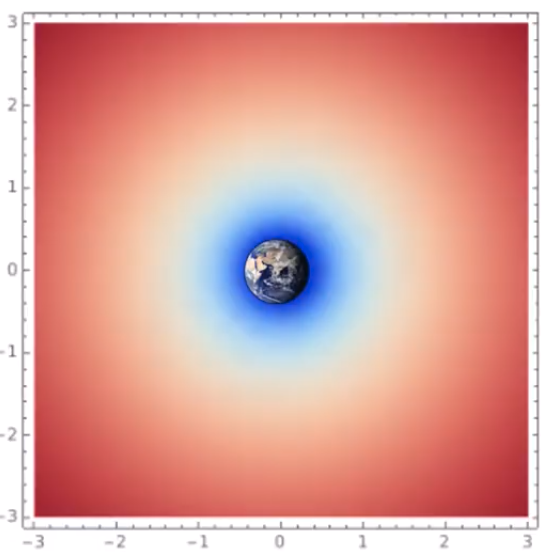
\includegraphics[scale=0.3]{figures/gravitational-potential.png}
\end{center}

Now using this definition of the gravitational force as dependning on the gradient of the gravitational potential, we can write, considering cartesian coordinates:

\begin{align*}
    W &= \int_{\begingroup\color{orange}P\endgroup} \begingroup\color{cyan}\vec{F}_G\endgroup \cdot \frac{d\begingroup\color{violet}\vec{R}\endgroup}{d\begingroup\color{brown}\lambda\endgroup} d\begingroup\color{brown}\lambda\endgroup\\
    &= \int_{\begingroup\color{orange}P\endgroup} m(-\grad{\begingroup\color{olive}\Phi\endgroup}) \cdot \frac{d\begingroup\color{violet}\vec{R}\endgroup}{d\begingroup\color{brown}\lambda\endgroup} d\begingroup\color{brown}\lambda\endgroup\\
    \grad{\begingroup\color{olive}\Phi\endgroup} &= \frac{\partial \begingroup\color{olive}\Phi\endgroup}{\partial \begingroup\color{cyan}x\endgroup} \begingroup\color{blue}\vec{e_x}\endgroup + \frac{\partial \begingroup\color{olive}\Phi\endgroup}{\partial \begingroup\color{cyan}y\endgroup} \begingroup\color{blue}\vec{e_y}\endgroup\\
    \frac{d\begingroup\color{violet}\vec{R}\endgroup}{d\begingroup\color{brown}\lambda\endgroup} &= 
    \frac{d\begingroup\color{cyan}x\endgroup}{d\begingroup\color{brown}\lambda\endgroup} \frac{d\begingroup\color{violet}\vec{R}\endgroup}{d\begingroup\color{cyan}x\endgroup} +
    \frac{d\begingroup\color{cyan}y\endgroup}{d\begingroup\color{brown}\lambda\endgroup} \frac{d\begingroup\color{violet}\vec{R}\endgroup}{d\begingroup\color{cyan}y\endgroup}\\
    &= \frac{d\begingroup\color{cyan}x\endgroup}{d\begingroup\color{brown}\lambda\endgroup} \begingroup\color{blue}\vec{e_x}\endgroup + \frac{d\begingroup\color{cyan}y\endgroup}{d\begingroup\color{brown}\lambda\endgroup}\begingroup\color{blue}\vec{e_y}\endgroup\\\\
    \grad{\begingroup\color{olive}\Phi\endgroup} &\cdot \frac{d\begingroup\color{violet}\vec{R}\endgroup}{d\begingroup\color{brown}\lambda\endgroup}\\
    &= \frac{\partial \begingroup\color{olive}\Phi\endgroup}{\partial \begingroup\color{cyan}x\endgroup}\frac{d\begingroup\color{cyan}x\endgroup}{d\begingroup\color{brown}\lambda\endgroup} +
     \frac{\partial \begingroup\color{olive}\Phi\endgroup}{\partial \begingroup\color{cyan}y\endgroup}\frac{d\begingroup\color{cyan}y\endgroup}{d\begingroup\color{brown}\lambda\endgroup}
\end{align*}

So that:

\begin{align*}
    W &= \int_{\begingroup\color{orange}P\endgroup} m(-\grad{\begingroup\color{olive}\Phi\endgroup}) \cdot \frac{d\begingroup\color{violet}\vec{R}\endgroup}{d\begingroup\color{brown}\lambda\endgroup} d\begingroup\color{brown}\lambda\endgroup\\
    &= -m \int_{\begingroup\color{orange}P\endgroup} \frac{d \begingroup\color{olive}\Phi\endgroup}{d \begingroup\color{brown}\lambda\endgroup}d\begingroup\color{brown}\lambda\endgroup\\
    &= -m \int_{\begingroup\color{orange}P\endgroup} d \begingroup\color{olive}\Phi\endgroup\\
    &= -m \left[\begingroup\color{olive}\Phi\endgroup(\begingroup\color{orange}P_{end}\endgroup) - \begingroup\color{olive}\Phi\endgroup(\begingroup\color{orange}P_{start}\endgroup)\right]
\end{align*}

So really, when we write down the integral with the dot product between the gradient and the tangent vectors along the curve, we're sort of overcomplicating things, 
because all of it is just the expaneded version of $d \begingroup\color{olive}\Phi\endgroup$.\\
We just have to evaluate $\begingroup\color{olive}\Phi\endgroup$ at the end and at the start of the curve and then subtract.\\

Looking at the scalar field and not the associated vector field (given by the gradient of the scalar field) does indeed make more sense to compute
the work.\\
Then, yet another way of looking at things, instead of looking at the scalar field $\begingroup\color{olive}\Phi\endgroup$, we can look at the level sets of $\begingroup\color{olive}\Phi\endgroup$, 
and when we draw a path through these level sets, if we can to compute the work along, we just look at where the path starts, where it ends, and see how much 
the function has changed. Basically by counting how many level sets, the path piereces from start to end.\\\\

We can move ahead with another of example, with a simple single variable integration.\\

\begin{align*}
   \int_{\begingroup\color{blue}0\endgroup}^{\begingroup\color{blue}2\endgroup} \begingroup\color{red}(-6x + 4)dx\endgroup
\end{align*}

Integration is over the single variable $x$.
If we represent this function and compute the integral as we are usually doing:

\begin{center}
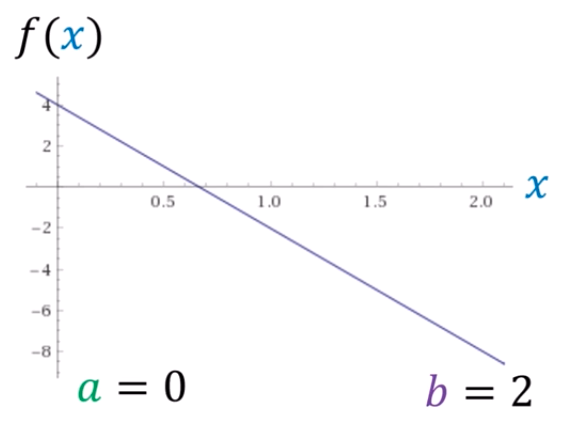
\includegraphics[scale=0.3]{figures/single-var-int.png}
\end{center}

\begin{align*}
    & \int_{\begingroup\color{blue}0\endgroup}^{\begingroup\color{blue}2\endgroup} \begingroup\color{red}(-6x + 4)dx\endgroup \\
    &= \left[\begingroup\color{red}-3x^2 + 4x\endgroup\right]_{\begingroup\color{blue}0\endgroup}^{\begingroup\color{blue}2\endgroup} \\
    &= \left[\begingroup\color{red}-3(2)^2 + 4(2)\endgroup\right] - \left[\begingroup\color{red}-3(0)^2 + 4(0)\endgroup\right] \\
    &= -12 + 8 \\
    &= -4
\end{align*}\\

We can think of re-interpreting this using our new covector field vision:

\begin{align*}
    & \int_{\begingroup\color{blue}0\endgroup}^{\begingroup\color{blue}2\endgroup} \begingroup\color{red}(-6x + 4)dx\endgroup \\
    &= \int_{\begingroup\color{blue}0\endgroup}^{\begingroup\color{blue}2\endgroup} \frac{d \begingroup\color{brown}F\endgroup}{d\begingroup\color{red}x\endgroup}d\begingroup\color{red}x\endgroup\\
    &= \int_{\begingroup\color{blue}0\endgroup}^{\begingroup\color{blue}2\endgroup} d \begingroup\color{brown}F\endgroup\\ \\
    & \frac{d \begingroup\color{brown}F\endgroup}{d\begingroup\color{red}x\endgroup} = -6 \begingroup\color{red}x\endgroup + 4\\
    & \begingroup\color{brown}F\endgroup(\begingroup\color{red}x\endgroup) = -3\begingroup\color{red}x^2\endgroup + 4\begingroup\color{red}x\endgroup + C
\end{align*}

Visualising it, it would look like this function here, but we can also visualize it as scalar field:

\begin{center}
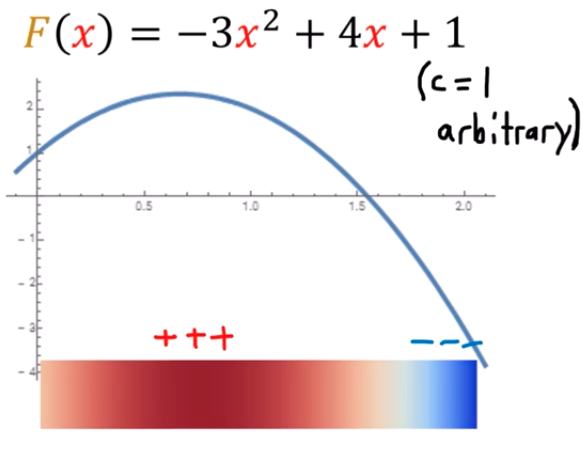
\includegraphics[scale=0.3]{figures/single-var-int-scalar.png}
\end{center}

The associated covector field $d\begingroup\color{brown}F\endgroup$ would look like this:

\begin{center}
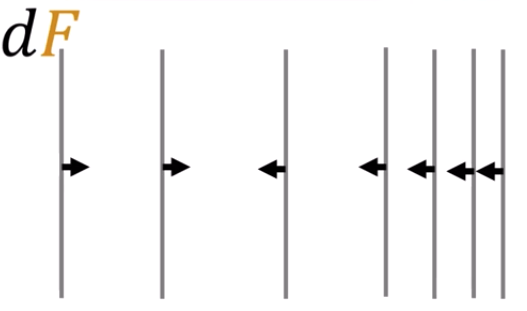
\includegraphics[scale=0.3]{figures/single-var-int-cov-field.png}
\end{center}

If you now plot the path from $x=0$ to $x=2$, you can clearly see yourself that, adding a +1 when 
the path pierces the covector field along its direction, and a -1 when on the opposite direction, the path
crosses the covector field exactly $+1 -1 -1 -1 -1 -1 = -4$ times, which is exactly the same value we got before using standard calculus.